L'ottica geometrica è una branca della fisica classica che permette di descrivere 
efficacemente la propagazione della luce, nell'approssimazione in cui la lunghezza d'onda $\lambda$ del raggio luminoso 
sia molto inferiore alle dimensioni $d$ degli ostacoli incontrati: 
\begin{center}
	$\lambda << d$
\end{center}
In tale contesto, la luce può essere rappresentata come un fascio di raggi rettilinei, 
ciascuno dei quali rappresenta la direzione di propagazione dell'onda luminosa. Si tratta di un modello semplificato che 
permette però di descrivere un'ampia gamma di fenomeni in maniera soddisfacente e senza ricorrere al concetto di onda. In un mezzo omogeneo e trasparente, la luce si propaga secondo traiettorie rettilinee. 
L'evidenza sperimentale mostra infatti che  un corpo opaco interposto tra una sorgente luminosa puntiforme e uno schermo, 
proietta un'ombra con contorni ben definiti, la cui forma dipende dalla geometria dell'ostacolo e dalla direzione dei raggi incidenti, 
compatibilmente con il principio secondo cui i raggi luminosi si propagano in linea retta e non possono aggirare gli ostacoli.
\begin{figure}[H]
	\centering
	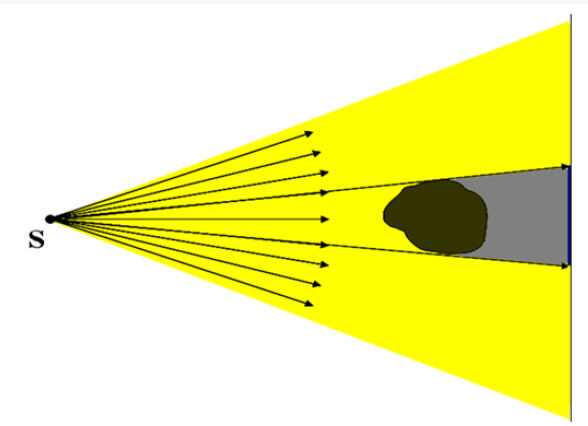
\includegraphics[width=0.55\textwidth]{./figures/cono-luce.png}
	\caption{La regione d’ombra, al di là
		dell’ostacolo è limitata al solo
		cono avente per vertice la sorgente
		puntiforme S e generatrici tangenti
		all’ostacolo.}
\end{figure}

Questo principio trova applicazione pratica nella camera oscura, in cui un piccolo foro praticato su una parete di una scatola chiusa, proietta un'immagine invertita di una sorgente 
luminosa esterna sulla parete opposta interna alla scatola.
\begin{figure}[H]
	\centering
	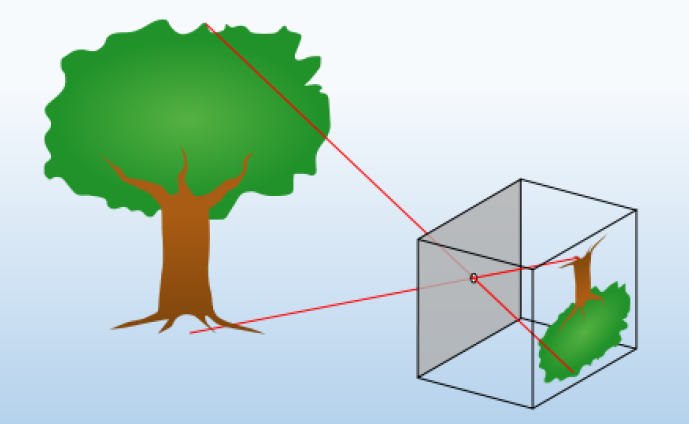
\includegraphics[width=0.55\textwidth]{./figures/camera_oscura.png}
	\caption{Camera Oscura}
\end{figure}

Sperimentalmente si osserva che quando un raggio luminoso attraversa l'interfaccia tra due mezzi, 
questo viene deviato rispetto alla normale alla superficie di separazione. Tale fenomeno è noto sotto il nome di \textbf{rifrazione}. é proprio a causa di questo fenomeno che possiamo osservare l'immagine spezzata di un oggetto immerso parzialmente in un bicchiere di acqua, come in figura. 
\begin{figure}[H]
	\centering
	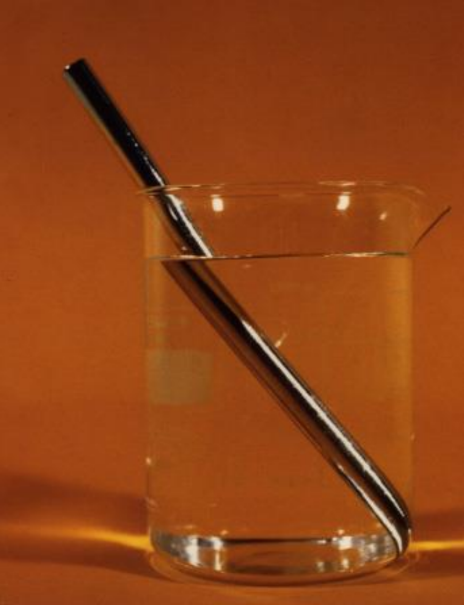
\includegraphics[width=0.55\textwidth]{./figures/img-spezzata.png}
	\caption{immagine spezzata di una matita parzialmente immersa in un bicchiere d'acqua}
\end{figure}
Il fenomeno della rifrazione è descritto dalla \textbf{Legge di Snell}, secondo la quale Il raggio incidente, quello rifratto e la normale alla superficie nel punto di incidenza, giacciono nello stesso piano:
\begin{equation}
    \frac{sin(\theta_i)}{sin(\theta_r)} = \frac{v_1}{v_2}
\end{equation}
Dove $\theta_i$ e $\theta_r$ sono gli angoli che il raggio luminoso forma con la normale alla superficie di incidenza nei rispettivi mezzi, mentre $v_1$ e $v_2$ sono le rispettive velocità di propagazione.
\begin{figure}[H]
	\centering
	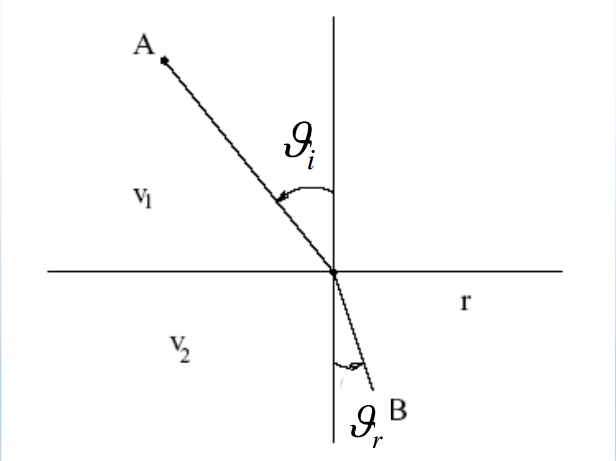
\includegraphics[width=0.55\textwidth]{./figures/rifrazione-1.png}
	\caption{}
\end{figure}
Si dicono inoltre:
\begin{enumerate}
    \item indice di rifrazione \textbf{assoluto}, il rapporto tra la velocità della luce nel vuoto e la velocità di propagazione nel mezzo: 
    \begin{equation}
        n = \frac{c}{v}
    \end{equation}
    \item indice di rifrazione \textbf{relativo} tra due mezzi $m_1$ ed $m_2$ il rapporto:
    \begin{equation}
        n_{21} = \frac{n_2}{n_1}
    \end{equation}
\end{enumerate}
Da quanto detto, si ricava grazie alla legge di Snell:
\begin{equation}
    \frac{sin(\theta_i)}{sin(\theta_r)} = \frac{v_1}{v_2} = \frac{n_2}{n_1}
\end{equation}
Da misure sperimentali risulta che l'indice di rifrazione assoluto dell'aria $n_1$ è pari ad 1, mentre quello dell'acqua $n_2$ è pari a 1,33. Dall'esperienza effettuata ci si attende pertanto un valore prossimo a 1,33.



\subsection{Richiami Statistici}
Il metodo dei minimi quadrati è una tecnica che permette di trovare una funzione, rappresentata da una curva di regressione, che si avvicini il più possibile ad un insieme di dati (tipicamente punti del piano). In particolare, la funzione trovata deve essere quella che minimizza la somma dei quadrati delle distanze tra i dati osservati e quelli della curva che rappresenta la funzione stessa. Siano $b$ il coefficiente angolare e $a$ l'intercetta della retta di regressione:
\begin{equation}
	b=\frac{\displaystyle\sum_{i=1}^{N}[(x_i-\overline{x})(y_i-\overline{y})]}{\displaystyle\sum_{i=1}^{N}(x_i-\overline{x})^2}
\end{equation}
\begin{equation}
	a=\overline{y}-b\overline{x}
\end{equation}
Con $\overline{x}=\frac{\displaystyle\sum_{i=1}^{N}x_i}{N}$ e $\overline{y}=\frac{\displaystyle\sum_{i=1}^{N}y_i}{N}$
mentre le incertezze:
\begin{equation}
	\Delta b=3\sigma_b
\end{equation}
\begin{equation}
	\Delta a=3\sigma_a
\end{equation}
Con $$\sigma_b=\sigma_y\sqrt{\frac{N}{\Delta}}$$
$$\sigma_y=\sqrt{\frac{\displaystyle\sum_{i=1}^{N}(y_i-bx_i-a)^2}{N-2}}$$
$$\sigma_a=\sigma_y\sqrt{\frac{\displaystyle\sum_{i=1}^{N}x_i^2}{\Delta}}$$
$$\Delta=N\displaystyle\sum_{i=1}^{N}(x_i-\overline{x})^2$$

\subsection{Richiami di teoria della misura}
Sia $g$ una grandezza fisica dipendente da $N$ grandezze fisiche $x_1,...,x_N$ tale che
\begin{equation}
	g=f(x_1,...,x_N)
\end{equation}
con
\begin{equation}
	x_1 = x_{1_0}\pm \Delta x_1
\end{equation}
$$ ... $$
\begin{equation}
	x_N = x_{N_0}\pm \Delta x_N
\end{equation}
La formula di propagazione dell'errore massimo è:
\begin{equation}
	\Delta g=\displaystyle\sum_{i=1}^{N}\left|\frac{\partial g}{\partial x_i}\right|_{\vec{x}=\vec{x_0}}\Delta x_i
\end{equation}
con
\begin{equation}
	\vec{x}=(x_1,...,x_N)
\end{equation}
\begin{equation}
	\vec{x_0}=(x_{1_0},...,x_{N_0})
\end{equation}

Sia $g$ una grandezza fisica pari alla somma, o alla differenza, di $N$ grandezze fisiche $x_1,...,x_N$ tale che
\begin{equation}
	g=x_1\pm ...\pm x_N
\end{equation}
con
\begin{equation}
	x_1=x_{1_0}\pm \Delta x_N
\end{equation}
$$ ... $$
\begin{equation}
	x_N=x_{N_0}\pm \Delta x_N
\end{equation}
La formula di propagazione dell'errore massimo è:
\begin{equation}
	\Delta g=\Delta x_1 + ... + \Delta x_N
\end{equation}